\documentclass[conference]{IEEEtran}
% This is stripped down to basically the ieee bare_conf.tex header
\usepackage{amssymb,amsmath}
% use upquote if available, for straight quotes in verbatim environments
\IfFileExists{upquote.sty}{\usepackage{upquote}}{}
% use microtype if available
\IfFileExists{microtype.sty}{%
\usepackage{microtype}
\UseMicrotypeSet[protrusion]{basicmath} % disable protrusion for tt fonts
}{}
\usepackage{hyperref}
\PassOptionsToPackage{usenames,dvipsnames}{color} % color is loaded by hyperref
\hypersetup{unicode=true,
            pdftitle={Identifying the True Origin of DNS Traffic Without Reference to Client Source Address},
            pdfborder={0 0 0},
            breaklinks=true}
\urlstyle{same}  % don't use monospace font for urls
% -- biblio. set natbib: true in pandoc for silly hacks around pandoc \cite{} vs \citep{}
\usepackage{cite}
\bibliographystyle{IEEEtran}
\let\citep\cite
% if you want the [2, 3] vs IEEE [2], [3]
\renewcommand{\citepunct}{,\penalty\citepunctpenalty\ }

\title{Identifying the True Origin of DNS Traffic Without Reference to Client
Source Address}
% author names and affiliations
% use a multiple column layout for up to three different
% affiliations
\author{\IEEEauthorblockN{Joe Abley}\IEEEauthorblockA{Western University, London, Ontario, Canada \\ Afilias Canada, Toronto, Ontario, Canada \\ \href{mailto:jabley@uwo.ca}{\nolinkurl{jabley@uwo.ca}},
\href{mailto:jabley@afilias.info}{\nolinkurl{jabley@afilias.info}}}}





\date{2018-12-08 00:12:34 -0500}
\setlength{\parindent}{0pt}
\setlength{\parskip}{6pt plus 2pt minus 1pt}
\let\tightlist\relax % silly pandoc thing

% --- user includes
% Put your preamble here. Example.
% subfigures
\usepackage{subfig}
% dots in filenames
\usepackage{graphicx, grffile}
% bold math
\usepackage{bm}
% colours
\usepackage[usenames,dvipsnames]{xcolor}
% suppress month in bibliography
%\AtEveryBibitem{\clearfield{month}}
%\AtEveryCitekey{\clearfield{month}}

% texdef -t latex -f {cmdname} to see if cmd is already defined

% Letters in fancy font (expectation, integers, reals, normal dist)
\newcommand{\E}[1]{\operatorname{\mathbb{E}}{\left[#1\right]}}
\newcommand{\Z}{\mathbb{Z}}
\newcommand{\R}{\mathbb{R}}
\newcommand{\N}{\mathcal{N}}

\begin{document}
\maketitle
\begin{abstract}
We demonstrate a model that is able to classify the originating system
responsible for stateless Domain Name System (DNS) queries received at
an authoritative DNS server without reference to source address. The
ability to determine whether particular DNS query traffic received at an
authoritative server is legitimately sourced from a particular client
system is useful in identifying various classes of malicious traffic in
production DNS systems.
\end{abstract}

\section{Introduction}\label{sec:introduction}

\label{sec:introduction}

The Domain Name System (DNS) includes a wire protocol with which
structured requests and responses are exchanged over a network. The DNS
protocol was originally specified \citep{rfc1034}\citep{rfc1035} for use
over both the Transmission Control Protocol (TCP) \citep{rfc793} and the
User Datagram Protocol (UDP) \citep{rfc768} and the use of other
transports have also been documented
\citep{rfc7858}\citep{rfc8484}\citep{huitema-quic-dnsoquic-05}. At
present, however, UDP is the overwhelmingly dominant transport protocol
in use; for example, according to statistics published by ICANN for
queries received at the L root server, UDP accounts for 98\% of all
queries
received.\footnote{\url{http://stats.dns.icann.org/plotcache/L-Root/transport_vs_qtype/2018-12-03T00:00-2018-12-03T23:59-all.html}}

Since UDP transport for DNS is stateless, consisting of single-datagram
queries and responses with no setup or tear-down handshake, there are
limited opportunities to verify the legitimacy of a source address. DNS
servers are consequently frequently used as amplifiers in reflection
attacks \citep{rfc5358}. Although some such attacks are trivially
identified, e.g.~by Query Type (QTYPE), many are more difficult. By
choosing query parameters that match legitimate, real-world use of the
DNS, attackers can make it difficult for their traffic to be identified
and blocked without causing collateral damage. This is especially true
of amplification attacks against DNS resolvers.

The clients of authoritative DNS servers are most usually DNS resolvers.
These client systems receive requests from end-user applications (or
downstream resolvers). Different client resolver systems are observed to
send different mixes of DNS traffic; for example, a resolver system that
mainly serves end-users will send a different mixture of queries to
authoritative servers than one which serves a specific application like
Internet mail \citep{rfc5321}, which might reasonably be expected to
have a much higher proportion of query traffic with \texttt{QTYPE=MX}.

Afilias Canada\footnote{\url{https://afilias.info/}} operates
authoritative DNS infrastructure for around 300 top-level domains,
including several that attract high levels of query traffic such as INFO
and ORG. This infrastructure is distributed globally using anycast
service distribution \citep{rfc4786}, using commodity transit services,
public peering and so-called Private Network Interconnects (PNIs). The
real origin of queries received over a PNI can be known with high
accuracy; the origin of queries received over the Internet, in contrast,
cannot. We refer to the former as \emph{trusted} paths, and the latter
as \emph{untrusted}. Trusted paths exist to Google Public
DNS,\footnote{\url{https://dns.google.com}} a public DNS resolver system
configured for use by a large number of end-users, and
Facebook,\footnote{\url{https://www.facebook.com}} whose resolver
systems are mainly used by back-end systems that build previews for
links shared between users of Facebook's social media platform. The
traffic patterns of each are expected to be usefully different.

While real-time anomoly detection in DNS traffic remains an elusive
problem, the ability to classify traffic apparently received by
particular sources as being legitimate is useful in the forensic
analysis of traffic spikes since it provides the opportunity to
distinguish between illegitimate, unwanted traffic and traffic from
clients that just happen to be busy, e.g.~due to a burst in popularity
in a particular web page, or changes in the Time To Live (TTL)
parameters of high-use domain names. This paper describes a system that
aims to provide such a classification.

We collected a raw DNS dataset in the form of individual (request,
response) DNS messages received from and sent to a single apparent
source over period of two weeks. We split the resulting query stream
into five minute intervals and from each we extract a vector of
variables that describes the traffic received from each client during
that time. Each such vector, once normalised, represents a single
observation related to a single client. Observations that correspond to
traffic received from the trusted sources, in this case Google and
Facebook, can be used as a training dataset. Observations corresponding
to DNS traffic that definitively did not arrive from a trusted source
can also be incorporated as ``other''. The resulting model can be used
to classify five-minute samples of query streams from purported single
sources to classify the origin of the query traffic as ``facebook'',
``google'' or ``other''. Since query sources for each category feature
in an equal number of traffic samples, it is straightforward to produce
a training dataset that is balanced across the three categories.

This paper is organised as follows. Section \ref{sec:introduction}
introduces the problem and provides some high-level background on the
DNS. Section \ref{sec:background} provides a short introduction to the
algorithms and accuracy measures that are used to build the model. Some
other work on applying machine learning techniques to problems in the
DNS are described in section \ref{sec:related}. Data collection and
preprocessing, feature engineering and choice of learning and validation
algorithms are discussed in section \ref{sec:methodology}. Section
\ref{sec:evaluation} describes the evaluation of the resulting model.
Section \ref{sec:conclusion} provides a summary of the work described in
this paper, and section \ref{sec:future} identifies some areas for
future study.

\section{Background}\label{sec:background}

\label{sec:background}

Two multiclass classifiers are evaluated for this model in section
\ref{sec:classifiers}, below. The approach used to evaluate the accuracy
of each is described in section \ref{sec:accuracy}. These models are
used to classify features of individual five-minute samples of DNS
reponse data according to source system by treating each sample as a
single observation. A brief discussion of other approaches that might
usefully consider each sample as a point along a time series can be
found in section \ref{sec:future}.

\subsection{Classifier Models}\label{sec:classifier-models}

\label{sec:classifiers}

We consider both Support Vector Machine and Random Forest models and
select the most successful one based on 10-fold validation.

\subsubsection{Multiclass Support Vector
Machine}\label{sec:multiclass-support-vector-machine}

\label{sec:svmmethod}

The classifier used in this paper was constructed as a series of Support
Vector Machines (SVM), each used as a binary classifier. SVM represents
\(n\)-dimensional support vectors in an \(n\)-axis hyperspace and
identifies a hyperplane boundary between observations known to be in
different categories to facilitate classification of unlabelled test
sets. Those boundaries can then be used to classify unlabelled
observations.

Multiclass classification is achieved using \(k(k-1)/2\)
\emph{one-against-one} binary classifiers combined with a max-wins
voting scheme, as discussed in \citep{10.1007/11494683_28}.

The SVM implementation used to construct this model exposes several
hyperparameters that can be tuned, as well as a native grid search to
assist identification of optimal parameters for a supplied validation
dataset.

\subsubsection{Random Forest}\label{sec:random-forest}

\label{sec:rfmethod}

Random Forests (RF) \citep{Breiman2001} combine many decision trees at
training time into an ensemble learning model. RF uses bootstrap samples
to introduce a random component into the tree-building process, whilst
also reducing correlation amongst trees, adding noise to perturb the
tree structure and using a random subset of available predictors each
each split. Each of \(m\) models in the resulting ensemble is used to
generate a prediction for a new sample and those predictions are
averaged to give the prediction from the entire forest.

The tuning parameters for the RF ensemble model are:

\begin{itemize}
\tightlist
\item
  the size of the subset of predictors randomly selected at each split,
  \(m_{try}\). Breiman suggests \citep{Breiman2001} setting \(m_{try}\)
  to be the square root of the number of predictors.
\item
  the number of trees in the forest. Breiman has proved that random
  forests are immune from overfitting, but but there might be some
  benefit in computational expense in limiting the size of the forest to
  the number of the trees that provides measurable benefit.
\end{itemize}

\subsection{Accuracy Measures}\label{sec:accuracy-measures}

\label{sec:accuracy}

We calculate a confusion matrix over a test dataset:

\begin{center}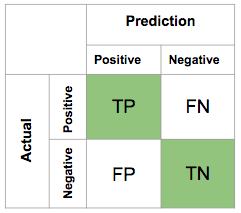
\includegraphics[width=0.5\linewidth]{confusion_matrix} \end{center}

Since we intend to ensure that we have a balanced dataset between the
three classifications of traffic samples, we are able to use a
straightforward measure of accuracy, A:

\[A = \frac{TP + TN}{TP + FP + TN + FN}\]

\section{Related Work}\label{sec:related-work}

\label{sec:related}

Machine learning techniques were applied to the problem of classifying
so-called core domains as part of a threat assessment in a production
system at
Nominum\footnote{Nominum was acquired by Akamai in November 2017}
\citep{Yuzifovichbotconf2017} \citep{YuzifovichOARC2017}. This problem
has some similarities to the problem described in this paper, and
illustrates the use of continuous learning to upadate an already-trained
model on arrival of new data.

The .NZ registry maintains a set of business intelligence datasets which
are constructed in part by analysis of queries received at authoritative
DNS servers. In order to improve the accuracy of those datasets, machine
learning techniques were used to build models that could classify query
sources as DNS resolvers or other systems (e.g.~systems performing
active monitoring of the DNS). The work included extensive feature
analysis and incorporated substantial domain knowledge derived from
earlier analysis. \citep{Qiao2018} \citep{QiaoOARC2018}.

A study in the application of different machine learning techniques was
presented in \citep{Sammour2017} as part of an attempt to train a model
to identify Internet traffic tunnelled over the DNS protocol.

The approach described in this paper differs from other approaches
described above in that it acknowledges the problems inherent in
grouping DNS transactions together without the ability to be certain
that the apparent sources of DNS queries are legitimate.

\section{Methodology}\label{sec:methodology}

\label{sec:methodology}

\subsection{Overview}\label{sec:overview}

\label{sec:methodology_overview} We collected a complete set of DNS
query data received with UDP transport over trusted and untrusted paths
at a major anycast site in Ashburn, VA,
USA.\footnote{This is a private dataset that the authors of this paper have authorisation to use.}
This source data is based on raw packet captures in PCAP
format,\footnote{PCAP, named after the C library \texttt{libpcap}, is the file format used by the \texttt{tcpdump} utility}
post-processed into \emph{dnscount} objects to extract various
parameters from the raw DNS messages: a timestamp; client and server
adresses (IPv4 and IPv6); the query type; query name; transport
protocol; response code; and DNS message flags. Separate \emph{dnscount}
objects are stored for queries and responses; the query objects differ
slightly in composition since they naturally do not include a response
code.

The \emph{dnscount} objects are centralised using
Redis\footnote{\url{https://redis.io/}} message brokers for integration
in other Afilias traffic measurement systems. Since the response objects
contain a superset of the information contained within the query objects
(they include a response code), and since they represent the results of
queries that are known to be well-formed to the extent that a nameserver
can produce a response, only the response objects for a sample period
were extracted for use in training this model. The production Redis
message brokers were not used since doing so would involve a release
engineering process which would introduce unnecessary cost and delay to
the collection process.

\subsection{Data Reduction}\label{sec:data-reduction}

The query summaries at this particular network site in Ashburn, VA
represent around 500GB of data per month when compressed using
bzip2,\footnote{\url{http://www.bzip.org/}} and hence an in-place
reduction and summarisation process was undertaken:

\begin{enumerate}
\def\labelenumi{\arabic{enumi}.}
\tightlist
\item
  Only data from the first week in November 2018 was considered. This
  seems intuitively like a long enough period to accommodate different
  workday and weekend behaviour without represending an unmaageable data
  set, although it seems intuitively true that a longer sample period
  would result in a better model (see also section \ref{sec:future});
\item
  Query \emph{dnscount} objects were discarded, since the corresponding
  response objects contain a superset (see section
  \ref{sec:methodology_overview});
\item
  Response objects with TCP transport were discarded, since transactions
  over an established TCP session have authenticated endpoint addresses
  through the TCP setup handshake;
\item
  Collections of the remaining objects within five-minute sample buckets
  were used to produce a set of summary observations for each (site,
  client, bucket), as described in section \ref{sec:datasetextraction}.
\end{enumerate}

The resulting summaries (compressed again using bzip2) occupied around
5GB, which is a more manageable data volume for transport over a network
to a central location. This data also contains no query names or client
(DNS resolver) IP addresses, allowing some confidence that it is free of
personally-identifiable information and hence presents no significant
threat to personal privacy.

\subsection{Feature Engineering}\label{sec:feature-engineering}

\label{sec:datasetextraction}

Individual \emph{dnscount} records were summarised in five-minute
intervals in order to characterise the nature of DNS traffic for the
corresponding (\emph{timestamp}, \emph{sitecode}, \emph{client}). The
resulting observations for each contained the following variables. These
were selected based on general domain knowledge about the DNS and about
the nature of the end-systems that trigger DNS queries to be sent from
Google and Facebook resolvers.

\begin{itemize}
\tightlist
\item
  (\emph{timestamp}, \emph{sitecode}, \emph{client})
\item
  number of responses counted in each five-minute sample interval
\item
  length of the largest observed label in all query name
\item
  the mean length of all observed labels in all query names
\item
  the number of unique top-level labels observed in all query names
\item
  the number of unique second-level domains observed in all query names
\item
  the proportion of query names that consisted of 1, 2, 3 or 4 labels
  (exposed as four separate variables)
\item
  the proportion of responses with response
  code\footnote{\url{https://www.iana.org/assignments/dns-parameters/dns-parameters.xhtml\#dns-parameters-6}}
  0 or 3 (two separate variables)
\item
  the proportion of responses with query
  type\footnote{\url{https://www.iana.org/assignments/dns-parameters/dns-parameters.xhtml\#dns-parameters-4}}
  1, 2, 5, 6, 15, 16, 28, 33, 35, 37, 38, 43, 44, 46, 48, 52, 99, 255,
  256, 257 and 32769 (twenty-one separate variables)
\end{itemize}

The query types chosen were those that appeared in the data and either
looked intuitively interesting or were frequently used. Frequently used
types include A (IPv4 address) and AAAA (IPv6 address); some types were
somewhat infrequent but were interesting: 32769 (DLV) and 33 (SRV) are
deprecated, for example, which makes them potentially more likely to
appear in the queries sent from a public resolver service like Google's
than a private one like Facebook's.

Datasets with the input variables described were further reduced for the
purposes of this experiment as follows:

\begin{enumerate}
\def\labelenumi{\arabic{enumi}.}
\tightlist
\item
  The day of the week and the hour of the day were extracted from the
  timestamp field, since all other components of the date seemed either
  too granular to allow any real correlation between different
  observations or invariant (e.g.~all observations were made in the same
  month and year).
\item
  The site code was discarded, since it's invariant across all
  observations in this dataset.
\end{enumerate}

These adaptations would not be applicable to datasets that included
observations over a longer time base, or from multiple sites.

Training and validation datasets were extracted from these summary sets
by collating all observations for each unique client observed in each
five-minute \emph{dnscount} sample, in the three cases:

\begin{enumerate}
\def\labelenumi{\arabic{enumi}.}
\tightlist
\item
  \emph{client} is known to be reachable via the Google PNI (candidate
  Google dataset);
\item
  \emph{client} is known to be reachable via the Facebook PNI (candidate
  Facebook dataset);
\item
  \emph{client} is not reachable via any PNI (candidate ``other''
  dataset).
\end{enumerate}

We choose particular clients in each category that demonstrate a
reasonable degree of activity, since it seems clear that an observation
that is based on a very small number of queries is unlikely to be very
useful as a predictor of query source: the patterns evident in the
observation will be correspondingly small. This selection process is
based on calculating the number of responses over the entire dataset for
all clients, sorting the resulting list and selecting active clients
that correspond to each of our three classifications.

Finally, the source datasets are reviewed in order to identify near-zero
variance predictors, and the corresponding predictors were eliminated.

\subsection{Validation Process}\label{sec:validation-process}

We validate each model described in section \ref{sec:classifiers} using
k-fold cross-validation over the training dataset with \(k=10\). This
provides an assessment of each model through ten folds of the source
data, giving a better measure of validation than a single
training/validation split.

The selected model is then trained over the entire training set, and
applied to the test set to measure the accuracy of its predictions, as
described in \ref{sec:accuracy}.

\section{Evaluation}\label{sec:evaluation}

\label{sec:evaluation}

\subsection{Software}\label{sec:software}

The implementations of SVM and RF used in this experiment were those
included in the
e1071\footnote{\url{https://cran.r-project.org/web/packages/e1071/}} and
randomForest\footnote{\url{https://cran.r-project.org/web/packages/randomForest/}}
libraries, respectively, used within
R\footnote{\url{https://www.r-project.org/}}. Data summarisation scripts
were written in POSIX sh and awk, and can be reviewed in the same
repository that holds the source of this document; see section
\ref{sec:colophon}.

\subsection{Data Preparation}\label{sec:data-preparation}

A dataset consisting of 2,895,503 observations of 35 predictor variables
was obtained as described in \ref{sec:datasetextraction}. These
observations were pre-classified as ``facebook'' (923,432 observations),
``google'' (1,954,409 observations) or ``other'' (17,212 observations).

For reasons that were not clear at the time of data collection, every
observation in the source dataset had appeared to be made on responses
with RCODE=0 (NOERROR) and none with RCODE=3 (NXDOMAIN) or any other
value. This is known not to be true, since if the DNS infrastructure
responsible for sending the responses counted in this dataset behaved
like that it would be a severe operational problem for the Internet.
Lacking any simple means to resolve whatever problem caused these
variables to carry false data, they were simply removed.

The \emph{responses} predictor was observed to have a small number of
large outliers which were not representative of the dataset as a whole.
Observations with \emph{response} values greater than a safe threshold
were removed.

The dataset exhibited a pronounced class imbalance; although the
observations classified as ``google'' and ``facebook'' were of roughly
the same number (within a factor of two) the ``other'' class was
substantially smaller: approximately 0.4\% of the size of the ``google''
class. Random-basis undersampling of the ``facebook'' and ``google''
classes was undertaken to reduce all three classes to the same size.

The \emph{responses}, \emph{hour}, \emph{max\_labelsize},
\emph{mean\_labelsize}, \emph{tlds\_seen} and \emph{slds\_seen}
predictors were rescaled within the range {[}0, 1{]} in order to match
the various \emph{prop}-named predictors.

The result of this process was a balanced, normalised dataset which was
split into a training dataset (75\%, 15,325 observations) and a test
dataset (25\%, 5,108 observations).

\subsection{Support Vector Machine}\label{sec:support-vector-machine}

A multiclass Support Vector Machine classifier was built using
C-classification and the RBF kernel, exposing the principal
hyperparameters \(\epsilon\) and \emph{cost}. A model was trained and
tuned using a grid search over those two parameters, resulting in a
tuned model with \(\gamma = 0.5\) and \(cost = 16\).

\begin{center}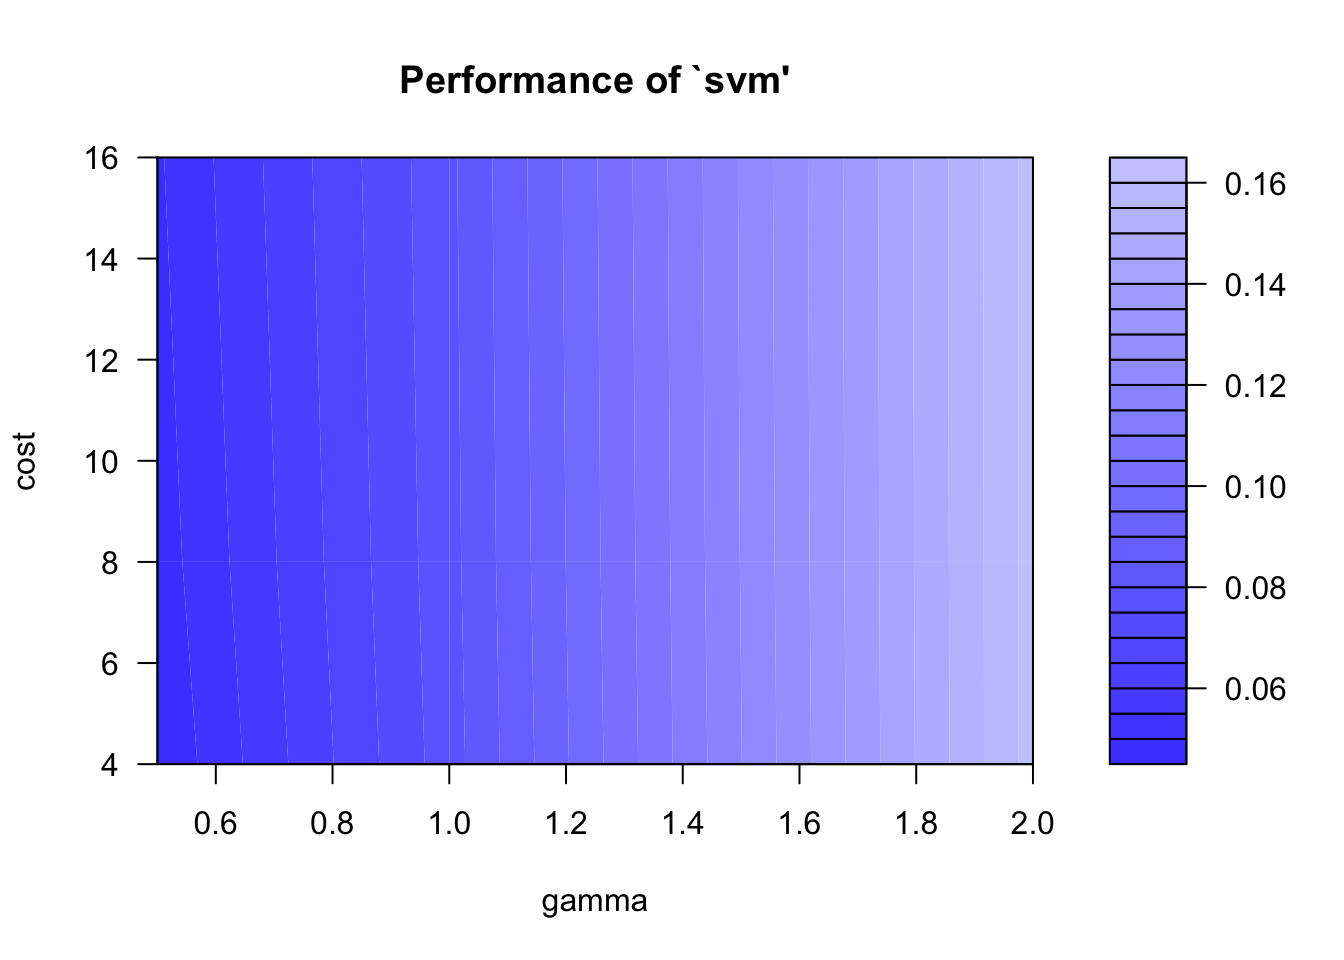
\includegraphics[width=1\linewidth]{SVM-tuning} \end{center}

10-fold cross-validation of the tuned model produced a mean accuracy
across all folds of 95.0299.

\subsection{Random Forest}\label{sec:random-forest-1}

A multiclass Random Forest classifier was built. The principal
hyperparameter available to tune is the number of trees in the forest;
it was observed that the chosen value of 500 seemed sufficient to ensure
stability in observed error. Random Forest does not suffer from
over-fitting as the number of trees increase and hence there was little
motivation to further constrain the forest size.

\begin{center}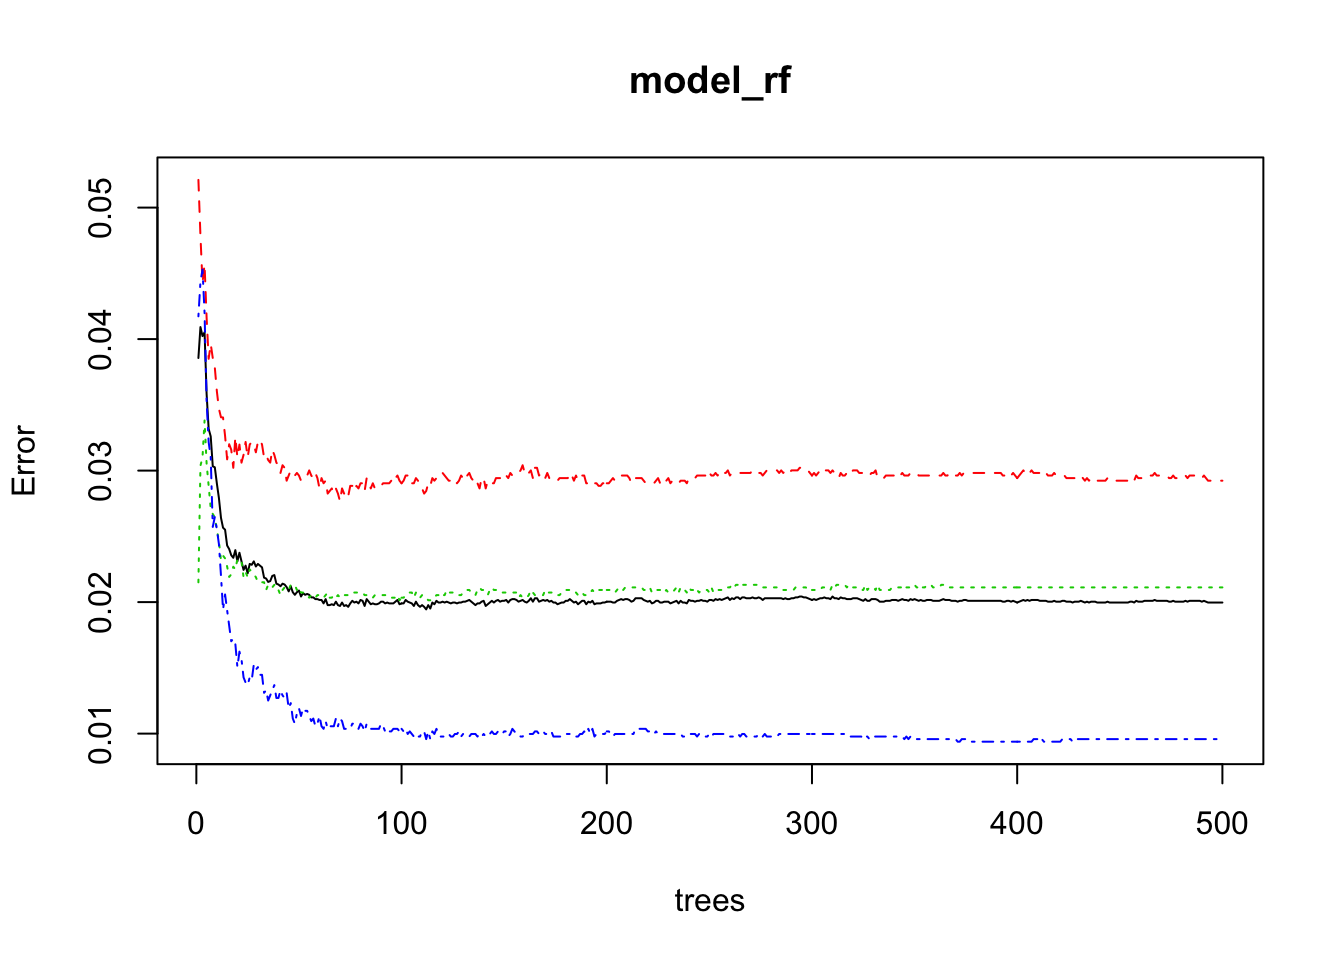
\includegraphics[width=1\linewidth]{RF-tuning} \end{center}

The implementation of Random Forest provides an OOB error rate which is
recommended for use instead of a cross-validation score. The OOB
estimate of the error rate in this case was 2\%.

\subsection{Accuracy Assessment}\label{sec:accuracy-assessment}

Each model was tested against the test dataset created as 25\% of the
observations in the source dataset, and a confusion matrix from each was
produced.

\subsubsection{Support Vector
Machine}\label{sec:support-vector-machine-1}

The accuracy of the SVM model is shown in the following confusion
matrix:

\begin{center}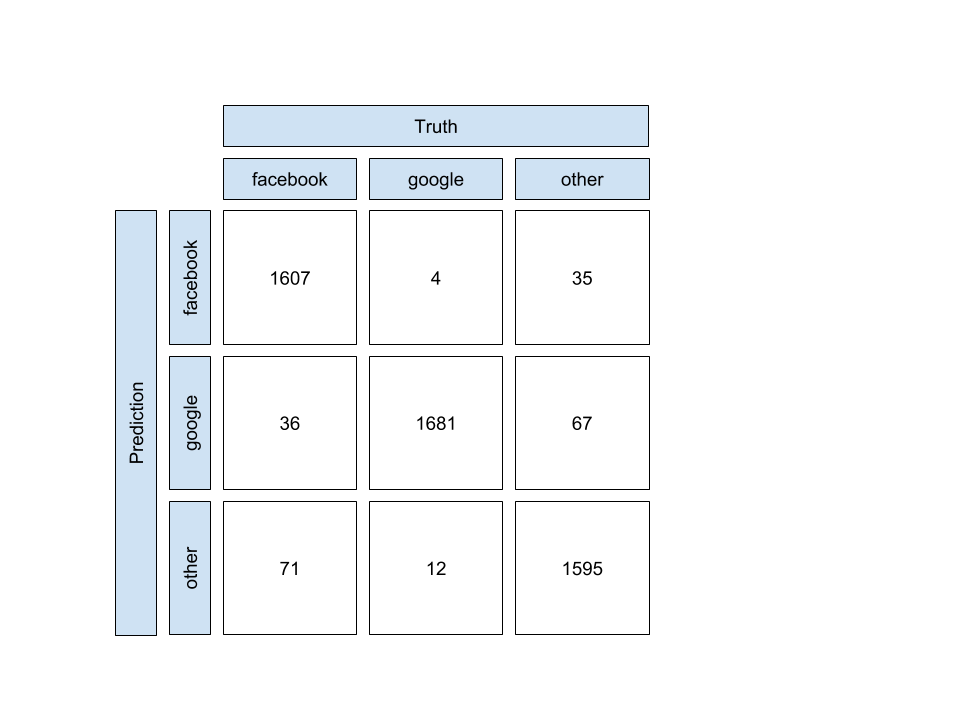
\includegraphics[width=1\linewidth]{SVM} \end{center}

Recall that:

\[A = \frac{TP + TN}{TP + FP + TN + FN}\]

The accuracy of the classifier can hence be represented as follows:

\[A_{facebook} = 0.9714\] \[A_{google} = 0.9936\] \[A_{other} = 0.9653\]

The SVM model exhibits high accuracy over the test set. Further study
would be required to validate its use as a general-purpose model;
fortunately there is no shortage of training data.

\subsubsection{Random Forest}\label{sec:random-forest-2}

The accuracy of the RF model is shown in the following confusion matrix:

\begin{center}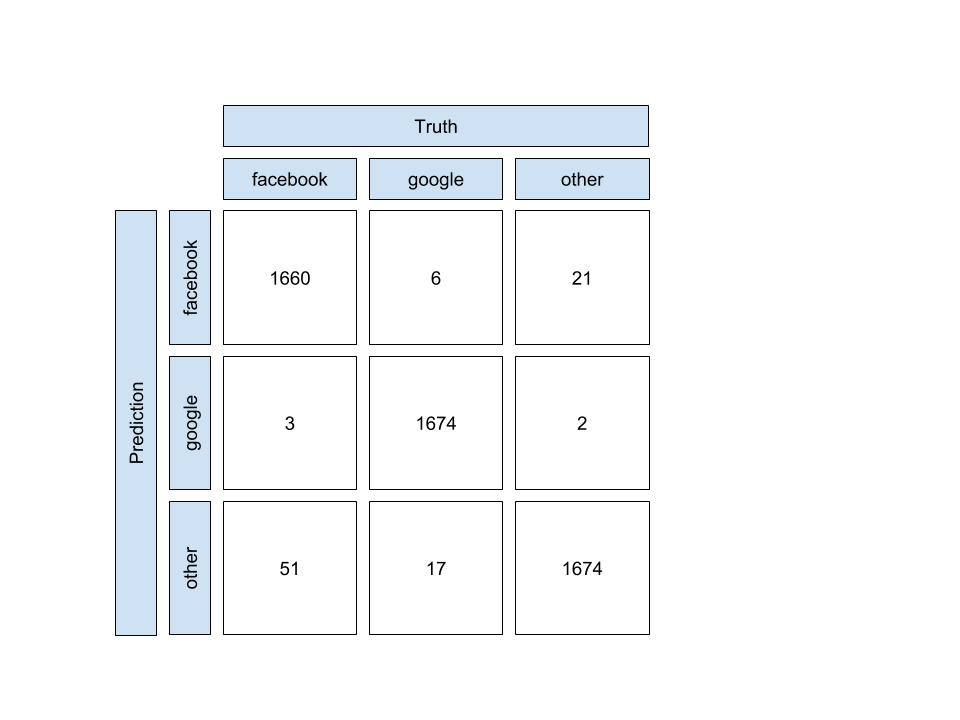
\includegraphics[width=1\linewidth]{RF} \end{center}

Again, recalling:

\[A = \frac{TP + TN}{TP + FP + TN + FN}\]

We obtain:

\[A_{facebook} = 0.9841\] \[A_{google} = 0.9945\]
\[A_{other} = 0.9822 \]

The RF model hence exhibits slightly higher accuracy over the test set,
and the same commentary as that over the SVM accuracy applies. It should
be noted that, at least in the implementations used in this paper,
Random Forests were far less computationally expensive over training
sets of the dimensionality seen here than Support Vector Machines,
perhaps because Random Forest lends itself more naturally to multi-class
problems.

\section{Conclusion}\label{sec:conclusion}

\label{sec:conclusion}

This paper aims to find a method that would allow a DNS query stream
received at an authoritative-only DNS server with UDP transport to be
classified as originating from DNS resolvers at Google, Facebook or
elsewhere, without reference to the IP source addresses of the queries.

Training datasets were created from five-minute samples of DNS traffic
captured off the wire at a single production Afilias DNS node,
responsible for serving around 300 top-level domains. Data reduction and
feature engineering were carried out, informed by both domain knowledge
and quantitative measures (e.g.~elimination of zero-variance
predictors). Two different classes of tuned model were built, one based
on Support Vector Machines and one on Random Forests. Both models
performed well, exhibiting a high degree of accuracy across a multitude
of measures.

The approach described and tested in this paper seems like a feasible
starting point for an operational system that could perform
near-real-time DNS traffic classification, providing capabilities such
as threshold alerting for traffic whose content appears not to match its
purported source.

\section{Future Study}\label{sec:future-study}

\label{sec:future}

This paper describes an assessment of two models, one based on Support
Vector Machines and one on Random Forests. These approaches were chosen
based on the ready availability of implementations and their reputations
for use in constructing supervised classifiers. It is certainly
possible, however, that a wider selection of models for assessment might
yield better approaches.

Three classifications were included in the datasets used in this
experiment. The specific source systems chosen, Facebook and Google,
were known to have different end-client populations and to have been
implemented using different DNS implementations. Additional exploration
of DNS data originating from other, less diverse client populations
would be useful to validate the general approach.

The features extracted from the source data relating to Query Names were
relatively unsophisticated, and seem unlikely to be capable of exposing
many patterns that might well be useful in characterising a particular
source system. Incorporating stronger string-similarity metrics might be
useful in exposing a measure of query entropy.

Using five-minute samples of query data is only suitable for clients
that send statistically-significant numbers of queries within that
sample interval. Increasing the sample interval (say, to an hour) might
allow less talkative clients to be assessed, but might also have an
impact on the observed variance in predictors between different classes.
A statistical approach to choosing a sample interval is likely better
than guessing.

Preparing datasets, centralising them and training and tuning models
took a significant amount of time. Much efficiency could be added using
conventional devops automation techniques, but a more scaleable approach
might well be found in finding an effective model that is amenable to
continuous learning. The data collection infrastructure deployed by
Afilias already facilitates data repatriation to a central location in
near real-time, and hence in-place, continuous training is at least
practical from a logistical perspective.

It is reasonable to expect that the grouping and ordering of DNS queries
might be relevant in the classification of a query stream as originating
from a particular DNS resolver. For example, the DNS Security Extensions
(DNSSEC) specification\cite{rfc4033} accommodates flexibility in the
order in which DNSSEC resource record sets are retrieved when a resolver
with an empty cache performs validation on an answer from a signed zone;
certain
applications\footnote{For example, qmail sends queries with QTYPE=ANY in an attempt to accelerate the process of retrieving answers that otherwise would require separate queries with QTYPE=A, AAAA and MX. The rarity of this approach was exposed when support for ANY queries on the server side started to become constrained. See \url{https://fanf.livejournal.com/122220.html} for related commentary.}
are also known to exhibit specific behaviour when using the DNS, and
resolvers that serve a community of such applications might exhibit
corresponding identifying behaviour. Particular web services use
signature combinations of content distribution network or embedded
advertiser beacons that might well provide a useful signature through a
resolver, even with the significant caching potential of answers
obtained from top-level domain authoritative nameservers. The models
described in this paper treat each query stream as an unordered set of
observations. The applicability of other models whose training can be
influenced by the ordering of data, e.g.~those based on recurant
multilayer perceptron networks, seem worthy of further investigation.

\section{Colophon}\label{sec:colophon}

\label{sec:colophon}

This document has been written in R
Markdown\footnote{\url{https://rmarkdown.rstudio.com}}; the code used to
produce the output included in this document is consequently included
with the document
source\footnote{\url{https://github.com/ableyjoe/uwo-mesc/tree/master/ECE-9603A-001-GF18/project}}.
The production of this document in IEEEtran style from R Markdown was
informed by a pseudonomymously-attributed community
project\footnote{\url{https://github.com/mathematicalcoffee/IEEEtran-rmarkdown}}.

\bibliography{IEEEabrv,./project}

\end{document}
